% %%%%%%%%%%%%%%%%%%%%%%%%%%%%%%%%%%%%%%%%%%%%%%%%%%%%%%%%%%%%%%%%%%%%%
% %% State-of-the-Art %%
% MatRaptor
% %%%%%%%%%%%%%%%%%%%%%%%%%%%%%%%%%%%%%%%%%%%%%%%%%%%%%%%%%%%%%%%%%%%%%

\subsection{MatRaptor}
\label{sec:soa:matraptor}

MatRaptor~\cite{Srivastava2020_MatRaptor} is an accelerator designed to compute SpMSpM kernels. It is based on \algo{Gust} algorithm\footnote{Called \emph{row-wise product} in~\cite{Srivastava2020_MatRaptor}.}, which makes it possible to process multiple $A$-rows (2 to 8 for MatRaptor) in parallel. In MatRaptor (see Figure~\ref{fig:soa:matraptor}) a \emph{SpAL} (\emph{Sparse Matrix A Loader}) fetches non-zero elements of a $A$-row and sends them to a \emph{SpBL} (\emph{Sparse Matrix B Loader}). With the \emph{metadata} of this element, the \emph{SpBL} fetches non-zero elements of the corresponding $B$-rows and sends pairs of $A$- and $B$-elements to a \emph{PE}. This \emph{PE} computes the \emph{partial sums} and sends the results into queues for the \emph{merge} process. Instead of separating \emph{multiply} and \emph{merge} phases, several queues are used to store \emph{partial sums} and partially merged \emph{partial sums}, allowing the two phases to be pipelined. The \emph{PE} merges all the \emph{partial sums} resulting from an entire $A$-row, before sending the final output (the corresponding $C$-row) to main memory.

In MatRaptor, multiple $A$-rows are processed independently and in parallel in different \emph{PEs} and each \emph{PE} is assigned to a channel in an HBM memory~\cite{JESD235B}. It is important that each \emph{PE} can read its $A$-rows without interfering with the other \emph{PEs}. With the classic \emph{(UOP, CP) row-major} format, the rows are consecutive in memory and are not aligned to channel boundaries. To solve this problem, the authors propose a new format called \emph{C$^2$SR} (\emph{(FL, UOP, CP) channel-major}) that is based on a \emph{(UOP, CP) row-major}. For example, with two \emph{PEs}, all the elements of the even rows are stored in one channel, and the elements of the odd rows, in another channel, thus isolating the data. With this approach, the row pointers (\emph{UOP}) are no longer monotonic, which means that the length of a row can not be deduced by subtracting adjacent row pointers. This requires the addition of a new table (which we call \emph{fiber length} \emph{FL}), which stores the length of the non-zero elements in each row (see Figure~\ref{fig:soa:C2SR}). This modified storage format enables multiple \emph{PEs} to make effective use of the HBM.

MatRaptor is one of the first accelerators to use \algo{Gust} algorithm, however, it has some limitations regarding effective reuse of $B$-rows, both between parallel \emph{SpBLs} and temporally, as $A$ is traversed. A key contribution is the proposed \emph{C$^2$SR} input format, which makes it possible to separate rows into memory channels, to improve performance.

\begin{figure}
    \centering
    \begin{minipage}[b]{0.34\linewidth}
        \begin{figure}[H]
            \centering
            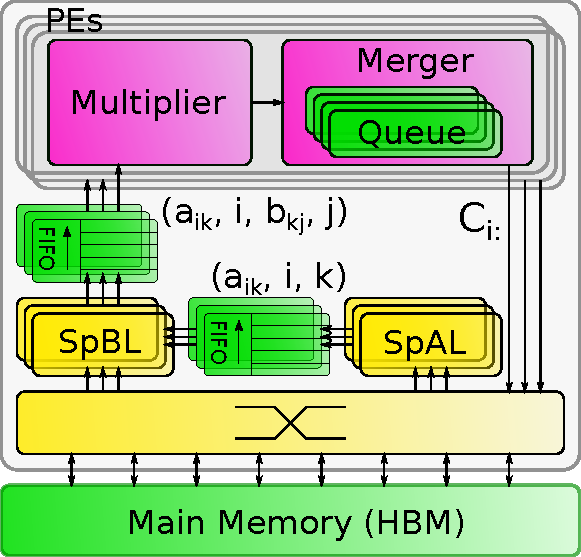
\includegraphics[width=0.85\textwidth]{Chapter_SoA/Figures/PDF/MatRaptor.pdf}
            \caption{Architecture of MatRaptor}
            \label{fig:soa:matraptor}
        \end{figure}
    \end{minipage}
    \hfill
    \begin{minipage}[b]{0.64\linewidth}
        \begin{figure}[H]
            \centering
            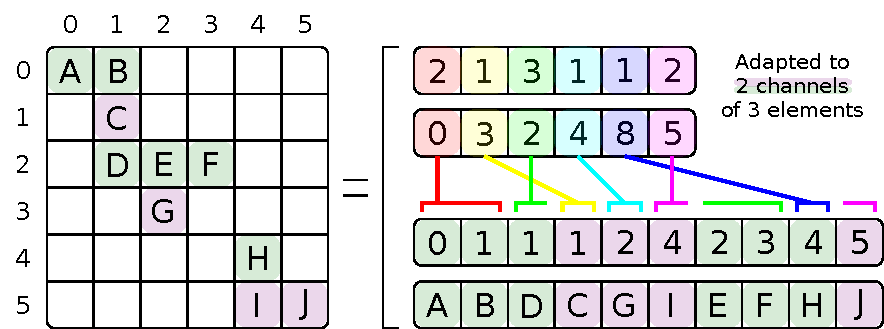
\includegraphics[width=0.9\textwidth]{Chapter_Background/Figures/PDF/SparseFormats/C2SR.pdf}
            \caption{\emph{(FL, UOP, CP) Channel-Major} Format ($C^{2}SR$)}
            \label{fig:soa:C2SR}
        \end{figure}
    \end{minipage}
\end{figure}